\documentclass[xcolor=dvipsnames]{beamer}


\newcommand\slideColor{Black}
%OliveGreen for meetings with Dr Roney	
%Mahogany for ECL meetings
%MidnightBlue for Beast meetings
%Black for Background meetings
%RedOrange for UVic meetings




\usepackage{xcolor}
\usepackage{hyperref}
\usepackage{multirow}
\usepackage{graphicx}
\usepackage{tikz}
\usepackage{url}
\usepackage{xcolor}
\usepackage[english]{babel}
\usepackage[latin1]{inputenc}
\usepackage{times}
\usepackage[T1]{fontenc}
\usepackage{xstring}
\usepackage{xparse}

\definecolor{dgreen}{rgb}{0.,0.6,0.}

\newcommand\defaultfon{\fontsize{11pt}{12}\selectfont}
\newcommand\smallfon{\fontsize{10pt}{12}\selectfont}
\newcommand\smallfontwo{\fontsize{8pt}{12}\selectfont}
\newcommand\smallfonthree{\fontsize{6pt}{12}\selectfont}
\newcommand\smallfonfour{\fontsize{6pt}{8}\selectfont}
\newcommand{\putat}[3]{\begin{picture}(0,0)(0,0)\put(#1,#2){#3}\end{picture}}

\newcommand\up{$\uparrow$}
\newcommand\down{$\downarrow$}





%To remove backup slides from count
\newcommand{\backupbegin}{
   \newcounter{finalframe}
   \setcounter{finalframe}{\value{framenumber}}
}
\newcommand{\backupend}{
   \setcounter{framenumber}{\value{finalframe}}
}

\mode<presentation>
{
  \usecolortheme[named=\slideColor]{structure}
  \usetheme{Madrid}

  
  \setbeamertemplate{navigation symbols}{} %remove navigation symbols
}

\institute[University of Victoria] 
{

\includegraphics[height=0.5in]{img/belle2-logo.pdf}\hspace{0.5cm}
\includegraphics[height=0.5in]{img/BeastLogo}\hspace{0.5cm}
\includegraphics[height=0.5in]{img/UVic_Logo}
 
  Department of Physics and Astronomy\\
  University of Victoria
}

\author[Samuel de Jong] 
{Samuel ~de Jong}




\title
{Simulation re-weighting scheme}

\subtitle
{applied to other BEAST II subdetectors} 

\author[Samuel de Jong] 
{Samuel ~de Jong}

%uncomment for meetings with mike
%\institute[University of Victoria] 


\date 
{\today}

\subject{BEAST II analysis}

\input{files}

\begin{document}

\begin{frame}
  \titlepage

\end{frame}

\newcommand*\oldmacro{}%
\let\oldmacro\insertshorttitle%
\renewcommand*\insertshorttitle{%
\vspace{-0.05cm}

\includegraphics[height=0.25cm]{img/belle2-logo.pdf}
\hspace{0.15cm}
\oldmacro% 
\hspace{0.15cm}

\includegraphics[height=0.25cm]{img/UVic_Shield}
%\hfill
}

%\begin{frame}{Outline}

  %\tableofcontents
  % You might wish to add the option [pausesections]
%\end{frame}

%START OF TALK
\section{Simulation weighting}

\subsection{Initial weighting}

\begin{frame}{Initial simulation weighting: beam gas}
\begin{itemize}
	\item
	The beam gas component was initial weighted:
	\begin{itemize}
		\item
		$R_{BG}^{Scaled} = \sum _{i=1}^{12}(R^{Brems}_i+R^{Coulomb}_i)\cdot\frac{(I\cdot P_i)} {(I\cdot P)_{sim}}$
	\end{itemize}
	\item
	Where the sum is over the 12 `D' sections where there is a pressure measurement.
	\item
	I modified this to include Z:
	\begin{itemize}
		\item
		$R_{BG}^{Scaled} = \sum _{i=1}^{12}(R^{Brems}_i+R^{Coulomb}_i)\cdot\frac{(I\cdot P_i\cdot Z_{i}^{2})_{data}} {(I\cdot P\cdot Z^{2})_{sim}}$
	\end{itemize}
	\item
	Where $Z_{sim}$=7, and $Z_{i}$ is Z measured in each `D' section if it is available. If it's not available, 2.7 is used for the LER, and 1 is used for the HER. 

\end{itemize}
\end{frame}


\begin{frame}{Initial simulation weighting: Touschek}
\begin{itemize}
	\item
	The Touschek component is weighted:
	\begin{itemize}
		\item
		$R_{Tous}^{Scaled} = R_{Tous}\cdot\frac{(I^{2}/N_{Bunch}\cdot\sigma_{y})_{data} }{(I^{2}/N_{Bunch}\cdot\sigma_{y})_{sim}}$	
	\end{itemize}
	\item
	This remains unchanged in my analysis.
	\item
	The simulated rate is then:
	\begin{itemize}
		\item
		$R_{Sim} = \left(R_{BG}^{Scaled}+R_{Tous}^{Scaled}\right)$
	\end{itemize}
		
\end{itemize}
\end{frame}


\begin{frame}{Fitting of data and simulation}
\begin{itemize}
	\item
	Now that weighted simulation ntuples are produced, I do some analysis on them.
	\item
	I fit the data and simulation to this equation:
	\begin{itemize}
		\item
		$R_{^{3}He\ tube} = c_{gas}\cdot P\cdot I\cdot Z^{2}+c_{T}\cdot \frac{I^{2}}{N_{Bunch}\cdot\sigma_{y}}$
	\end{itemize}
	\item
	with Z=1 for the HER, and the measurment of Z from D02 is used for the LER.
	\item
	The average pressure in the whole ring is used in this fitting.

\end{itemize}
\end{frame}


\begin{frame}{Comments in initial result}
\begin{itemize}
	\item
	There is large disagrement between data and simulation!
	\item
	We have been told there's a scaling factor of `3' on the pressure measurements, but I have no idea where this comes from or what the uncertainty is.
	\item
	Z is not 1 in the HER, but we have no way of knowing what it is, other than some measurements taken years ago

\end{itemize}
\end{frame}



\subsection{Reweighting}

\begin{frame}{Reweighting of simulation: beam-gas}
\begin{itemize}
	\item
	Let's introduce a scale factor on the Pressure, called $P_{scale}$
	\item
	Now I rescale the beam-gas simulation by:
	\begin{itemize}
		\item
		$R_{BG}^{Scaled} = \sum _{i=1}^{12}(R^{Brems}_i+R^{Coulomb}_i)\cdot\frac{P_{scale}(I\cdot P_i\cdot Z_{i}^{2})_{data}} {(I\cdot P\cdot Z^{2})_{sim}}$
	\end{itemize}
	\item
	I choose $P_{scale}$ so that the ratio of Touschek to beam-gas is the same in data as in simulation:
	\begin{itemize}
		\item
		$P_{scale} = \frac{(c_{gas}/c_{T})_{data}}{(c_{gas}/c_{T})_{sim}}$
	\end{itemize}
	\item
	The Touschek weighting is not changed.

\end{itemize}
\end{frame}

\begin{frame}{PScale: HER}
\begin{figure}	
	\includegraphics[height=2.5in]{../figs/Results/HERPScale}
\end{figure}
\end{frame}

\begin{frame}{PScale: LER}
\begin{figure}	
	\includegraphics[height=2.5in]{../figs/Results/LERPScale}
\end{figure}
\end{frame}

\begin{frame}{Fitting of data and reweighted simulation}
\begin{itemize}
	\item
	The data and simulation are fit to the same equation as before:
	\begin{itemize}
		\item
		$R_{^{3}He\ tube} = c_{gas}\cdot P\cdot I\cdot Z^{2}+c_{T}\cdot \frac{I^{2}}{N_{Bunch}\cdot\sigma_{y}}$
	\end{itemize}
	\item
	with Z=1 for the HER, and the measurment of Z from D02 is used for the LER.
	\item
	The average pressure in the whole ring is used in this fitting.

\end{itemize}
\end{frame}


\begin{frame}{Some interpretation}
\begin{itemize}
	\item
	The simulation looks a lot better now.
	\item
	The data and simulated rates are not equal to each other, but that's not a problem.
	\item
	$P_{scale}$ has very different values for the HER and LER:
	\begin{itemize}
		\item
		In the LER, Z is known, so $P_{scale}$ is just a scale in pressure
		\item
		In the HER, Z is not known, so $P_{scale}$ should really be called $P_{scale}Z^2$
	\end{itemize}	
	\item
	This analysis is discussed in Section 8.2 of my thesis: \href{https://www.dropbox.com/s/jji6kuvv6u854s7/mainthesisUVIC.pdf?dl=0}{\color{blue}{Dropbox link}}

\end{itemize}
\end{frame}

\section{Data/Sim Comparison}

\begin{frame}{Data - simulation comparison}
\begin{itemize}
	\item
	Define a ratio of data to simulation:
	\\ \Large
	$(D/S)_{gas} = c_{gas}^{data}/c_{gas}^{sim}$\\ \vspace{0.25cm}
	$(D/S)_{T} = c_{T}^{data}/c_{T}^{sim}$\\

\end{itemize}
\end{frame}

\begin{frame}{Data/Sim: HER}
\begin{figure}	
	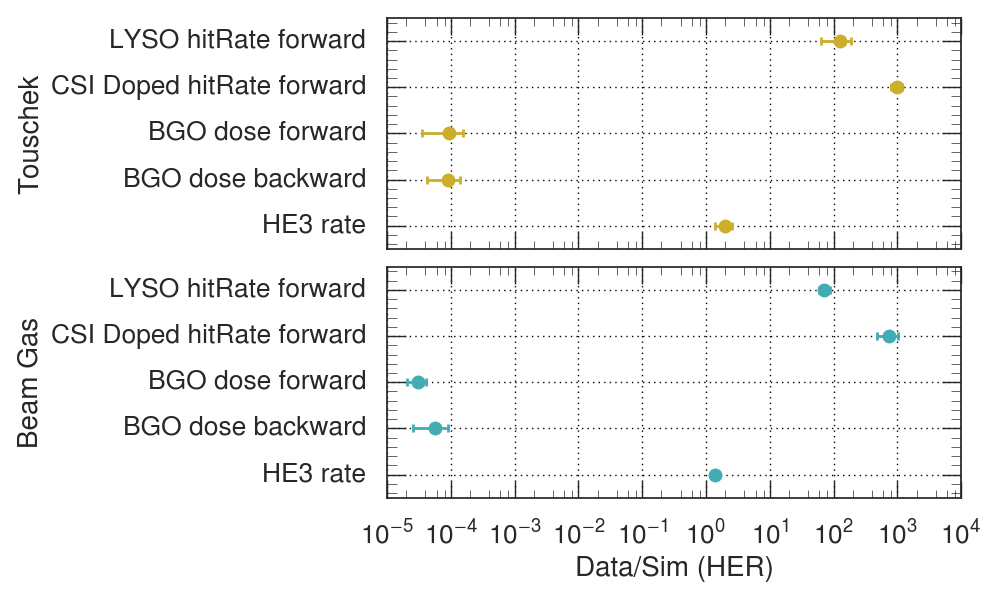
\includegraphics[height=2.5in]{../figs/Results/HERRatioPlot}
\end{figure}
\end{frame}

\begin{frame}{Data/Sim: LER}
\begin{figure}	
	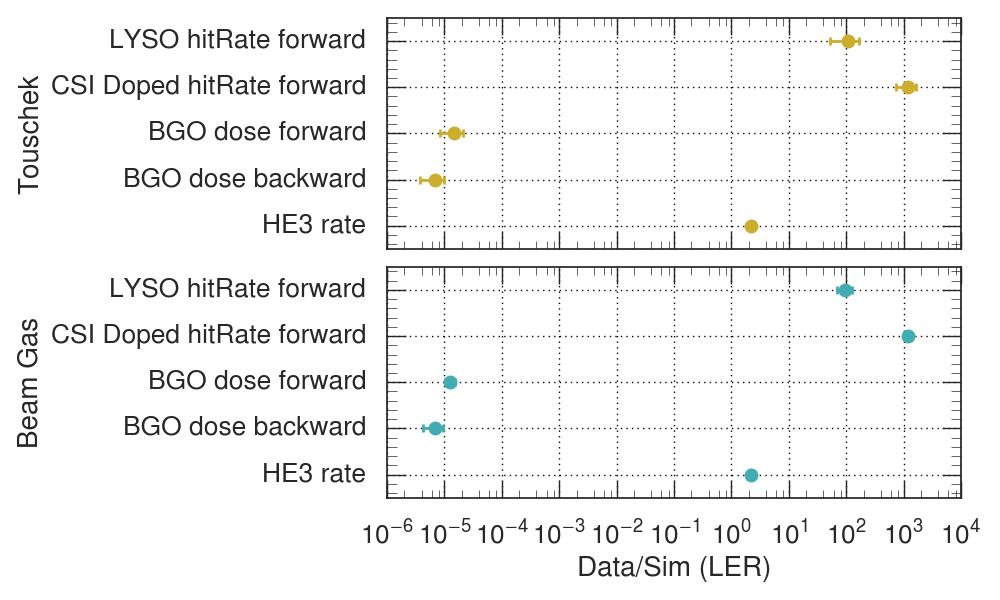
\includegraphics[height=2.5in]{../figs/Results/LERRatioPlot}
\end{figure}
\end{frame}

\appendix
\backupbegin
%Backup slides here

\begin{frame}
\begin{center}
\Huge Fitting results
\vspace{0.5cm}
\normalsize
\begin{itemize}
	\item
	On the graph slides, click on the slide title to go to a table with the fit values.
	\item
	On the table slides, click on a channel number to go to the associated graph.
\end{itemize}
\end{center}
\end{frame}


\foreach \c in \ListOfFiles {
	\IfSubStr{\c}{/}{	

		\expandarg
		\StrBehind[3]{\c}{/}[\temp]          
		\StrBefore[1]{\temp}{-}[\tempt]
		
		\section{\temp}

		\begin{frame}{\hyperlink{\tempt}{\StrSubstitute{\temp}{_}{ }}}
		\label{\temp}
		\begin{figure}	
			\includegraphics[height=3in]{"\c"}
		\end{figure}

		\end{frame}
	}{
		\input{\c}
	}
}


\backupend

\end{document}


